\documentclass{article}
\usepackage[utf8]{inputenc}
\usepackage{graphicx}
\usepackage{listings}
\usepackage[margin=2.5cm]{geometry}
\usepackage{tikz}
\usepackage{array}
\newcolumntype{L}[1]{>{\raggedright\let\newline\\\arraybackslash\hspace{0pt}}m{#1}}
\newcolumntype{C}[1]{>{\centering\let\newline\\\arraybackslash\hspace{0pt}}m{#1}}
\newcolumntype{R}[1]{>{\raggedleft\let\newline\\\arraybackslash\hspace{0pt}}m{#1}}
\usepackage{color}

\definecolor{dkgreen}{rgb}{0,0.6,0}
\definecolor{gray}{rgb}{0.5,0.5,0.5}
\definecolor{mauve}{rgb}{0.58,0,0.82}

\lstset{language=C,
  numbers=left,
  stepnumber=1,    
  firstnumber=1,
  numberfirstline=true
  aboveskip=5mm,
  belowskip=5mm,
  showstringspaces=false,
  columns=flexible,
  basicstyle={\small\ttfamily},
  numberstyle=\tiny\color{gray},
  keywordstyle=\color{blue},
  commentstyle=\color{dkgreen},
  stringstyle=\color{mauve},
  breaklines=true,
  breakatwhitespace=true
  tabsize=3
}



\title{{\bf Artificial Intelligence 1} \\ Lab $3a$}%Update the lab (assignment number)
\author{
Lennard Manuel (s number 1) \& Ethan Waterink (s number 2) \& Robbin de Groot (s number 3) \\
public\_static\_void\_main() \\
Learning Community 8
} %Change the names and fill in the student numbers, the learning community number and the team name

\date{day-month-year}%Update the date


%%%%%%%%%%%%%%%%%%%%%%%%%%%%%%%%%%%%%%%%%%%%%%%%%%%%%%%%%

\begin{document}

\maketitle

\section*{Exercise 1}
\subsection*{1.1 \hspace*{0.3cm} Solving a small set of equations}
\subsection*{1.2 \hspace*{0.3cm} Market}
\subsection*{1.3 \hspace*{0.3cm} Chain of trivial equations}
The constraint on every variable is that it must be equal to its predecessor, except for the first variable \verb|A|. Therefore, once we know the value of variable $v_{i-1}$, we have only one possible value for variable $v_i$ (where $1 \leq i \leq 26$). We can then show that inductively that every variable is equal to the first one, so $v_j = v_1$ where $2\leq j \leq 26$. This leaves us with a free variable, which we can set however we like. There are a total of $100$ possibilities, and therefore, $100$ solutions, since we don't run into any contradictions while setting the remaining variables. We can say that this technique is efficient, because whenever we set the first, unconstrained variable in the chain, there is exactly one solution. There is no need to branch off in two or more directions (in an imaginary tree structure), since the constraints only allow for one value on every variable. Therefore, every variable is set immediately, and is also correct. We recieve the expected results from the solver, as it finds $100$ solutions, and visits $2601$ states, which is minimal for this amount of solutions ($100\times 26=2600$).\\
In \verb|chainA.csp|, we do not have the choice of a free variable anymore. Previously, we had a chain of variables, with a free variable at the beginning. Now, that variable has been set to one specific value, due to the added constraint. This constraint will ripple down to the following variables, the same way as explained before. Therefore, only $1$ solution. The effectiveness boils down to the same as we said before, but since we have the extra constraint at the beginning of the chain, we do not evaluate any invalid states, and find set all variables correctly immediately.\\
In \verb|chainZ.csp|, the added constraint is on the last variable. This means that as we set our single free variable at the beginning of the chain, we only run into an issue, once we have gotten to the end of it, where there won't be any values left for \verb|Z| (if the chosen variable does not match the constraint). The effectiveness on this constraint is lower. There is only one solution, yet the solver has to visit a lot more states, since the extra constraint only becomes a problem at the end of the chain, after which we have to backtack all the way, and retry.\\
When running the solver, first with MRV, we notice contradictory results. In fact, the results we expected from \verb|chainA.csp| are recieved when running \verb|chainZ.csp| and vice versa. This means that our assumption, that the first declared variable is also the first to be evaluated is wrong; it is the last one. Therefore, the results are opposite of what we predicted. This `surpise' was foreshadowed in the introduction of the exercise, where we are told that results of seemingly identical descriptions might yield more or less efficient results. Moreover, for all 3 \verb|.csp|-files, the results are identical, no matter what propagation technique is used.

\subsection*{1.4 \hspace*{0.3cm} Cryptarithmetic puzzles}
\begin{tabular}{L{1.7cm}|L{13cm}}
Problem & Most effective algorithm + explanation\\\hline
\verb|MONEY| & ARC is most effective on its own, but combined with MRV, finds a solution by only visiting 40 states. This is most likely, because both techniques operate around the amount of available values for each variable. ARC removes the redundant ones, and MRV uses the remaining values to decide what state to set next. This combination does not have to be fast in all possible cases, but this specific combination proves to be solved very easily using these two techniques. \\\hline
\verb|ONZE| & The best technique for this problem is ARC. It alone solves the problem by visiting 58 states. An explanation for this could be that, in comparison with \verb|MONEY|, this problem has fewer variables with more possible values and more `words'. This allows ARC to eliminate more values for each variable, since there are more relations between fewer nodes. \\\hline
\verb|EIGHTY| & This one proves more difficult to solve. The fastest results are (again) given by the combination of MRV and ARC. This totals $1227$ visited states. Other singles or combinations of techniques don't even get remotely close to this. As stated before, ARC seems to operate best which a lot of relations, and in some cases, MRV can take a lot of advantage of that. \\\hline
\verb|HURTS| & Most techniques yield fast results, except for MRV and combinations of. It seems that is this specific case, MRV is not able to reduce the amount of possible values per variable all that quickly. This leads to a bigger search tree. We also see the degree heuristic performing well for a change. The fact that there are a lot of `words', and thus a lot of connections per letter, allows it to rule out a lot of options quickly. For example, the word ``I'' has connections to 3 other variables. As well as that, this puzzle has words that all have about the same letter in them, the most prominent being ``S'', ``T'' and ``H''. Therefore, these are all tied together by a lot of constraints, which DEG can take advantage of.\\
\end{tabular}

\subsection*{1.5 \hspace*{0.3cm} Finding the first 20 primes}
Arc consistency seems to be the only technique to solve the problem reasonably quickly. The combination of degree heuristic and forward checking also seems to work, but it takes about 5 seconds to do so ($524289$ states visited). \\
ARC is effective because primes are numbers that are \textit{not} related to others by means of multiplication. Because ARC only applies constraints between two nodes, it can rule out options extremely quickly, since there is no need to check with other (unrelated) nodes to begin with. So to conclude, arc consistency works best, because the relations involved in the definition of prime numbers is identical to the one of arc consistency.
\subsection*{1.6 \hspace*{0.3cm} Solving sudokus}
\subsection*{1.7 \hspace*{0.3cm} $n$-queens problem (again)}

\section*{Exercise 2}
\subsection*{2.1 \hspace*{0.3cm} Constraint Graph}
\subsection*{2.2 \hspace*{0.3cm} Magic Squares}
A magic square has the following prerequisites:
\begin{itemize}
    \item Every number in each grid square has a unique value from $1$ to $n^2$
    \item All rows, columns and both diagonals have an equal sum.
\end{itemize}
Using these definitions, we can set up a CSP description.\\
Clearly, we need $n^2$ variable, and one variable to store the value every row, column and diagonal has to be equal to. We make an array \verb|v[16]| and a variable \verb|a| for these. The domain for \verb|v|, are the values between 1 and 16. \verb|a| is any value between the maximum and minimum, which are $1+2+3+4=10$ and $13+14+15+16=58$. We know that the value that \verb|a| will take is unique, and in case of $n=4$ is $34$, but we assume we do not know this.\\
The constraints are simple. We need all values int \verb|v| to be different, so \verb|alldiff(v);|, and the sum of each row, column and diagonal to be equal to \verb|a|, so \verb|v[0] + v[1] + v[2] + v[3] = a; ....|. Finally, we want all solutions, so \verb|solutions: all;|. The final csp-file looks like:
\begin{verbatim}
variables:
  a,v[16]: integer;
domains:
  a <- [10..56]; v <- [1..16];
constraints: 
  alldiff(v);
# horizontals
  v[0] + v[1] + v[2] + v[3] = a;
  v[4] + v[5] + v[6] + v[7] = a;
  v[8] + v[9] + v[10] + v[11] = a;
  v[12] + v[13] + v[14] + v[15] = a;
# verticals
  v[0] + v[4] + v[8] + v[12] = a;
  v[1] + v[5] + v[9] + v[13] = a;
  v[2] + v[6] + v[10] + v[14] = a;
  v[3] + v[7] + v[11] + v[15] = a;
# diagonals
  v[0] + v[5] + v[10] + v[15] = a;
  v[3] + v[6] + v[9] + v[12] = a;
solutions: all
\end{verbatim}
Running the program using the MRV combined with ARC takes about 10 minutes to terminate, and finds 7040 solutions. What follows is the last snippet of the output.
\begin{verbatim}
### Solution 7037 ###
a =   34 
v =   13 12 8 1 7 2 14 11 10 15 3 6 4 5 9 16 

### Solution 7038 ###
a =   34 
v =   13 12 8 1 11 2 14 7 6 15 3 10 4 5 9 16 

### Solution 7039 ###
a =   34 
v =   13 12 8 1 10 3 15 6 7 14 2 11 4 5 9 16 

### Solution 7040 ###
a =   34 
v =   13 12 8 1 6 3 15 10 11 14 2 7 4 5 9 16 

Number of visited states: 3891179
Number of solutions: 7040
\end{verbatim}
This output means that, if we take solution 7040 as an example, the square would look like this
\begin{center}
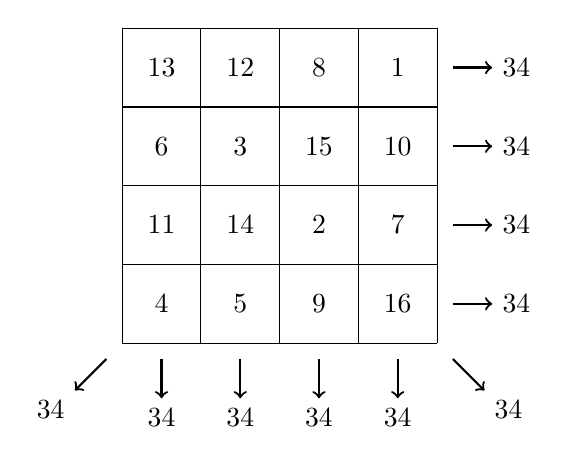
\begin{tikzpicture}
\draw (0,0) grid (4,4);
\node at (0.5,3.5) {13};
\node at (1.5,3.5) {12};
\node at (2.5,3.5) {8};
\node at (3.5,3.5) {1};
\node at (0.5,2.5) {6};
\node at (1.5,2.5) {3};
\node at (2.5,2.5) {15};
\node at (3.5,2.5) {10};
\node at (0.5,1.5) {11};
\node at (1.5,1.5) {14};
\node at (2.5,1.5) {2};
\node at (3.5,1.5) {7};
\node at (0.5,0.5) {4};
\node at (1.5,0.5) {5};
\node at (2.5,0.5) {9};
\node at (3.5,0.5) {16};
\draw[thick,->] (4.2,3.5) -- (4.7,3.5) node[anchor=west] {34};
\draw[thick,->] (4.2,2.5) -- (4.7,2.5) node[anchor=west] {34};
\draw[thick,->] (4.2,1.5) -- (4.7,1.5) node[anchor=west] {34};
\draw[thick,->] (4.2,0.5) -- (4.7,0.5) node[anchor=west] {34};
\draw[thick,->] (0.5,-0.2) -- (0.5,-0.7) node[anchor=north] {34};
\draw[thick,->] (1.5,-0.2) -- (1.5,-0.7) node[anchor=north] {34};
\draw[thick,->] (2.5,-0.2) -- (2.5,-0.7) node[anchor=north] {34};
\draw[thick,->] (3.5,-0.2) -- (3.5,-0.7) node[anchor=north] {34};
\draw[thick,->] (4.2,-0.2) -- (4.6,-0.6) node[anchor=north west] {34};
\draw[thick,->] (-0.2,-0.2) -- (-0.6,-0.6) node[anchor=north east] {34};
\end{tikzpicture}
\end{center}
We found that there are in fact 880 unique solutions to this problem, disregarding any rotations and mirrors of the same solution. This means this amount solutions is correct, since $(4\times2)\times880=7040$.
\subsection*{2.3 \hspace*{0.3cm} Boolean Satifiability}

\section*{To include code in your report use this}
\begin{lstlisting}[title=\textbf{Main.c}]
Your code here
\end{lstlisting}

\begin{lstlisting}[title=\textbf{Somefile.c}]
Some other code here
\end{lstlisting}

\end{document}